\newpage
\appendix
\onecolumn

\section{Visualization of Thermometer Encoding Effects} \label{app:thermo_effects}

As shown in \cref{fig:thermo_bird}, the thermometer-encoded channels lose most color information and only retain partial edge information. Further, only a small portion of channels contain non-trivial and non-overlapping information; in most cases, merely a single channel retains label information, up to repetition. This phenomenon inspires our hypothesis in \cref{sec:exp_convolution}.
\begin{figure*}[!htbp]
    \centering
    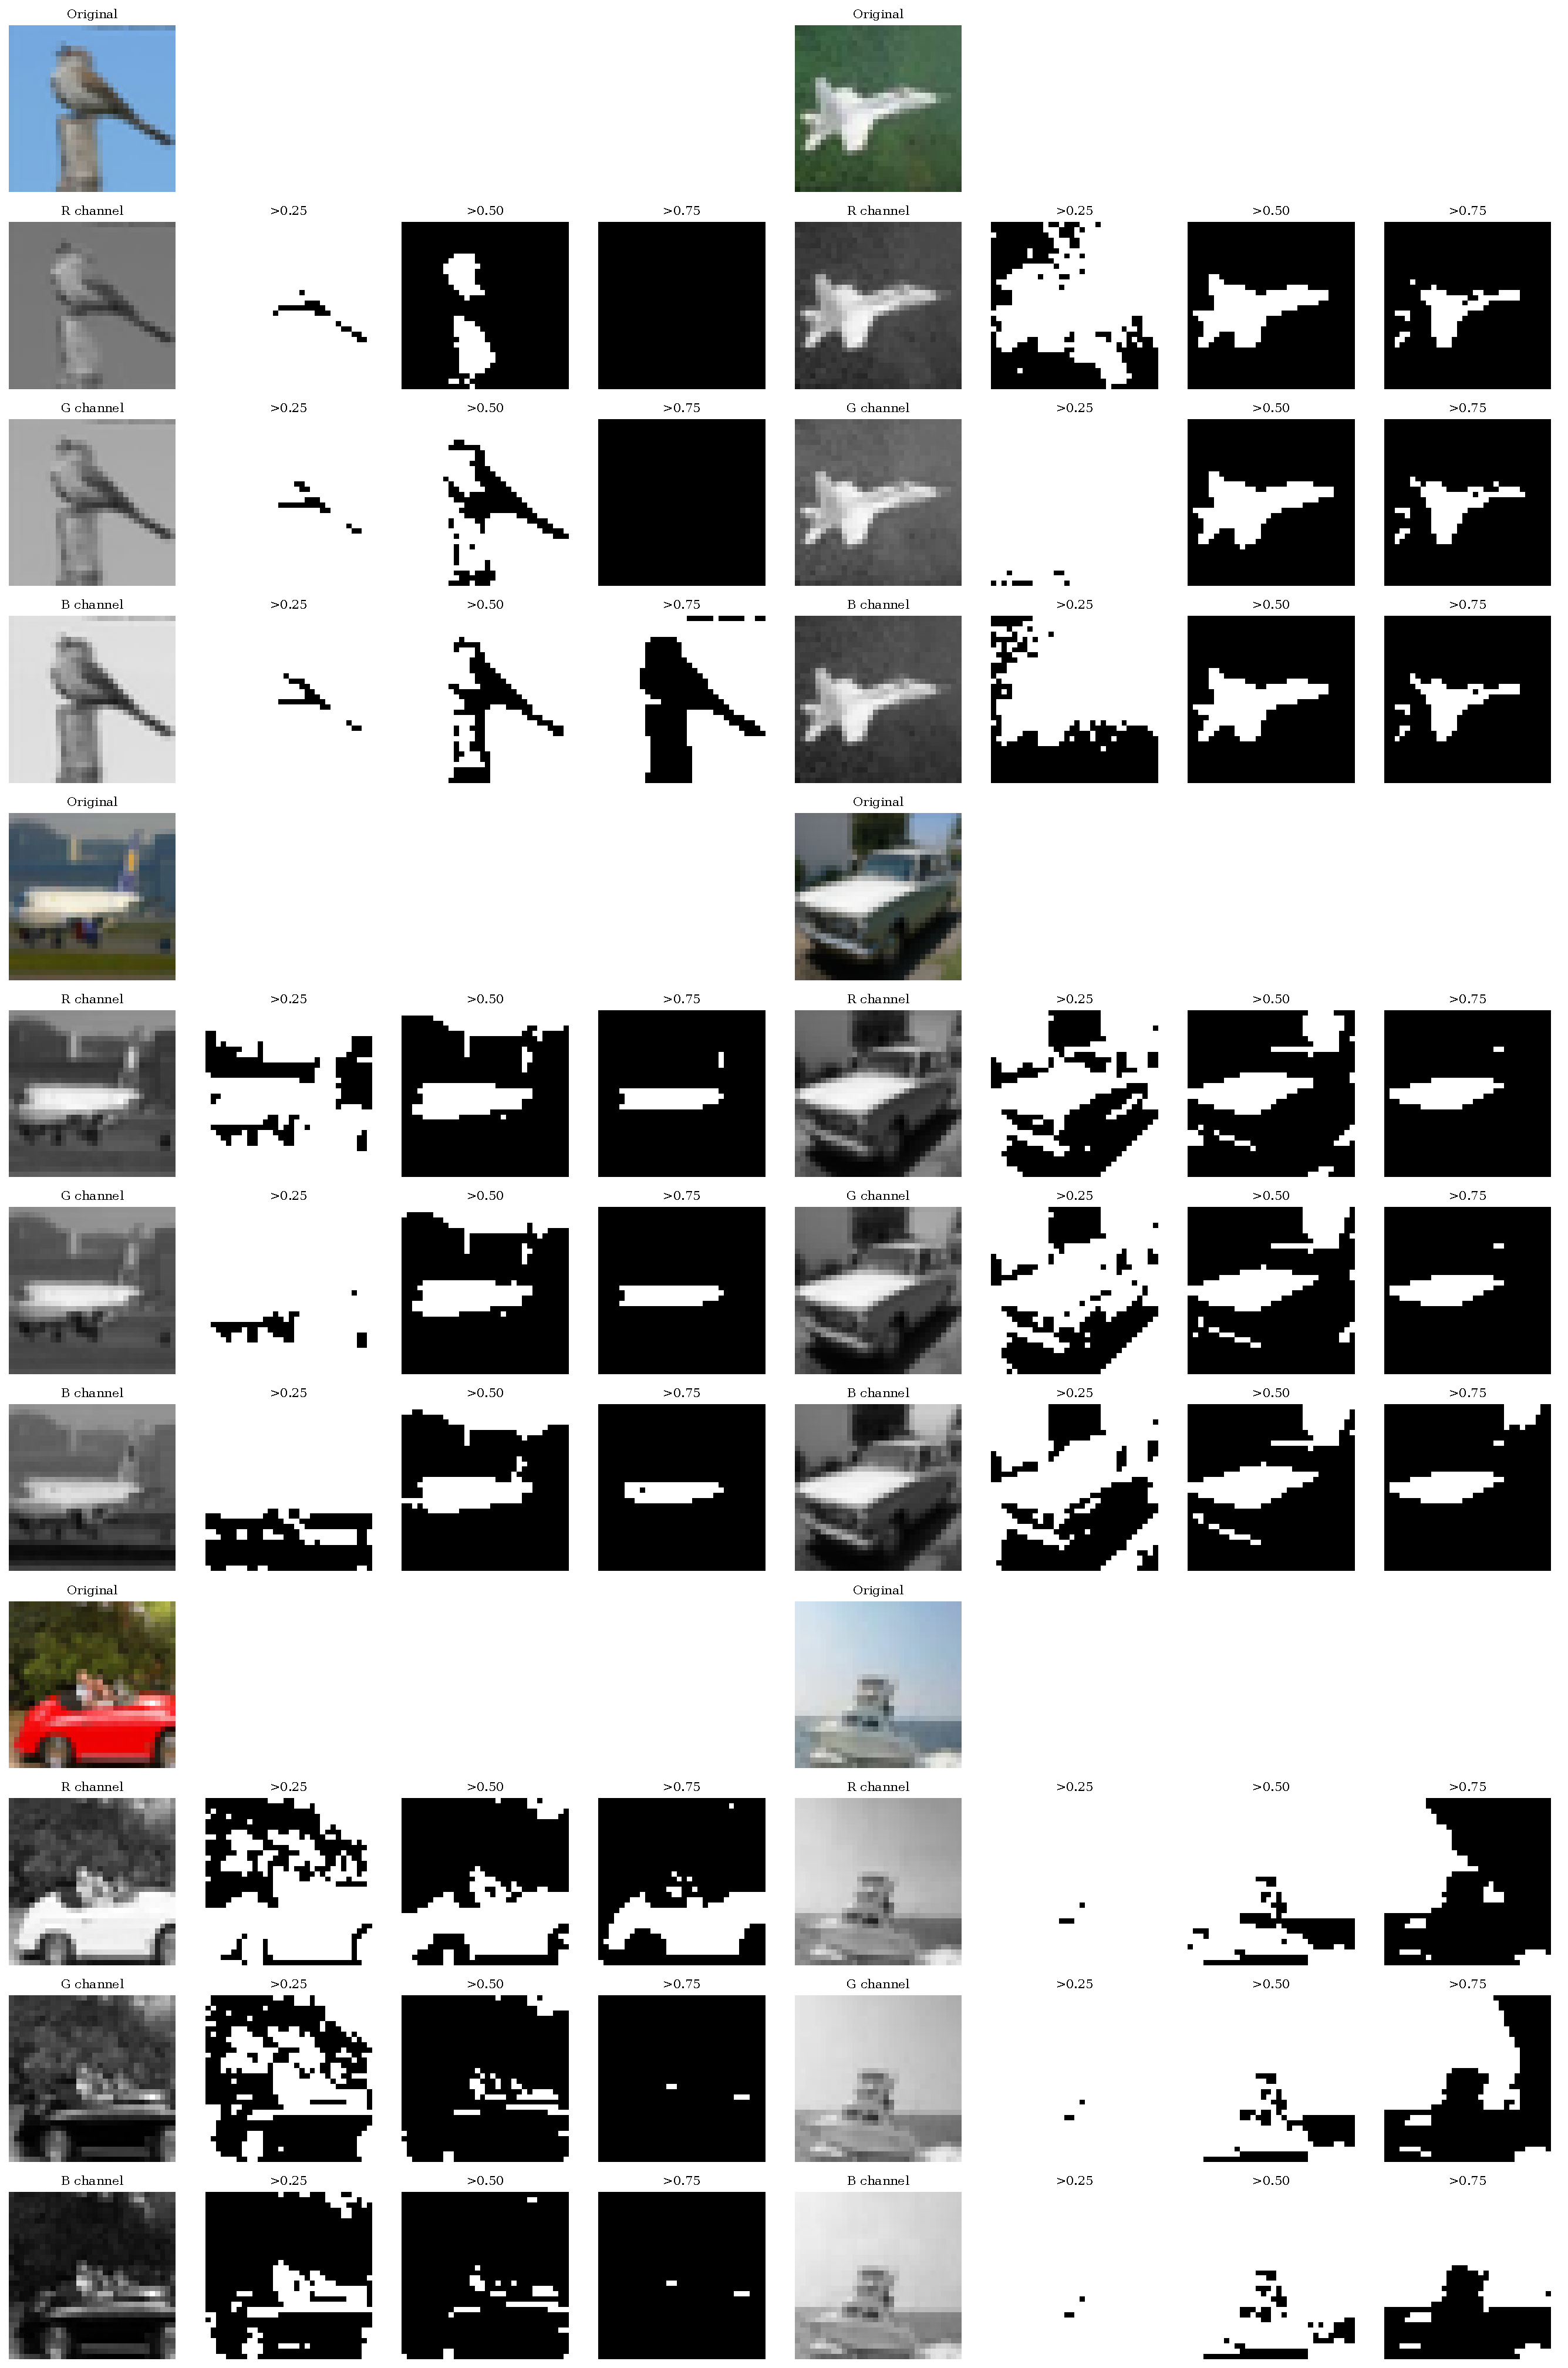
\includegraphics[width=0.72\linewidth]{figures/thermo_bird}
    \caption{Illustration of the destructive effect of thermometer encoding on the channels of natural images from \cifar.}
    \label{fig:thermo_bird}
\end{figure*}

\section{Variance Across Random Seeds} \label{app:variance_seeds}

To verify the stability of our methods, we repeat the main results in \cref{sec:exp_connection} and \cref{sec:exp_convolution} with different random seeds and report the mean and standard deviation in \cref{tb:DLGN_MNIST_rs}, \cref{tb:DLGN_CIFAR_rs}, \cref{tb:CLGN_MNIST_rs}, and \cref{tb:CLGN_CIFAR_rs}, respectively. Results show that our method consistently outperforms the baselines with a clear margin under different random seeds, demonstrating the robustness of our approach.

\begin{table}[!htbp]
\centering
\caption{Statistics on \mnist for connection learning.}
\label{tb:DLGN_MNIST_rs}
\begin{tabular}{lccc}
\toprule
Method & Acc. & \emph{\#neurons} & \emph{\#BOPs} \\
\midrule
DiffLogicNet (small)    & $97.03\% \pm 0.10\%$ & 48.0 K & 27.0 $\pm$ 0.1 K \\
DiffLogicNet (medium)   & $98.78\% \pm 0.02\%$ & 384 K & 215 $\pm$ 1 K \\
\midrule
Ours (small)            & \textbf{$97.77\% \pm 0.13\%$} & 48.0 K & 25.2 $\pm$ 0.4 K \\
Ours (medium)           & \textbf{$99.06\% \pm 0.03\%$} & 384 K & 190 $\pm$ 1 K \\
\bottomrule
\end{tabular}
\end{table}

\begin{table}[!htbp]
\centering
\caption{Statistics on \cifar for connection learning.}
\label{tb:DLGN_CIFAR_rs}
\begin{tabular}{lccc}
\toprule
Method & Acc. & \emph{\#neurons} & \emph{\#BOPs} \\
\midrule
DiffLogicNet (small)    & $52.70\% \pm 0.15\%$ & 48.0 K & 27.0 $\pm$ 0.7 K \\
DiffLogicNet (medium)   & $59.74\% \pm 0.11\%$ & 512 K & 311 $\pm$ 1 K \\
DiffLogicNet (large)    & $61.48\% \pm 0.76\%$ & 1.28 M & 780 $\pm$ 2 K \\
\midrule
Ours (small)            & \textbf{$55.81\% \pm 0.33\%$} & 48.0 K & 27.6 $\pm$ 0.3 K \\
Ours (medium)            & \textbf{$62.46\% \pm 0.27\%$} & 512 K & 296 $\pm$ 2 K \\
Ours (large)            & \textbf{$64.16\% \pm 0.26\%$} & 1.28 M & 655 $\pm$ 1 K \\
\bottomrule
\end{tabular}
\end{table}

\begin{table}[!htbp]
\centering
\caption{Statistics on \mnist for convolution.}
\label{tb:CLGN_MNIST_rs}
\begin{tabular}{lccc}
\toprule
Method & Acc. & \emph{\#neurons} & \emph{\#BOPs} \\
\midrule
TreeLogicNet-S    & $97.76\% \pm 0.04\%$ & 220 K & 120 $\pm$ 1 K \\
TreeLogicNet-M    & $98.87\% \pm 0.12\%$ & 883 K & 433 $\pm$ 2 K \\
TreeLogicNet-L    & $99.28\% \pm 0.03\%$ & 11.8 M & 6.20 $\pm$ 0.03 M \\
\midrule
Ours-S            & \textbf{$99.33\% \pm 0.01\%$} & 260 K & 168 $\pm$ 2 K \\
Ours-M            & \textbf{$99.34\% \pm 0.07\%$} & 520 K & 259 $\pm$ 3 K \\
\bottomrule
\end{tabular}
\end{table}

\begin{table}[!htbp]
\centering
\caption{Statistics on \cifar for convolution.}
\label{tb:CLGN_CIFAR_rs}
\begin{tabular}{lccc}
\toprule
Method & Acc. & \emph{\#neurons} & \emph{\#BOPs} \\
\midrule
TreeLogicNet-S    & $59.47\% \pm 0.35\%$ & 874 K & 538 $\pm$ 8 K \\
TreeLogicNet-M    & $71.30\% \pm 0.06\%$ & 7.00 M & 3.76 $\pm$ 0.06 M \\
\midrule
Ours-T	& \textbf{$62.24\% \pm 0.07\%$} & 145 K & 100 $\pm$ 1 K \\
Ours-S	& \textbf{$66.74\% \pm 0.18\%$} & 291 K & 191 $\pm$ 12 K \\
Ours-M	& \textbf{$69.90\% \pm 0.24\%$} & 582 K & 374 $\pm$ 26 K \\
Ours-L	& \textbf{$72.33\% \pm 0.23\%$} & 2.33 M & 1.08 $\pm$ 0.12 M \\
\bottomrule
\end{tabular}
\end{table}




















\section{Implementation for TreeLogicNet} \label{app:convlogic}

Since \citet{petersen2024convolutional} did not release the official implementation of TreeLogicNet, we use a community implemented version available at \citet{korinek_convlogic}. To verify the correctness of this implementation, we compare the test accuracies obtained from the GitHub implementation and those reported in \citet{petersen2024convolutional}. The results are summarized in \cref{tb:convlogic}. While the reported accuracies from the community implementation are slightly lower than those reported in \citet{petersen2024convolutional}, we find that simply applying the same data augmentation strategy as in our experiments during training closes the performance gap. This partially confirms the correctness of the community implementation, allowing us to use it as a baseline for convolutional Boolean networks in our experiments.

\begin{table}
\centering
\caption{A comparison between the reported accuracy from \citet{petersen2024convolutional} and the community implemented TreeLogicNet (named ConvLogic).}
\label{tb:convlogic}
\resizebox{0.7\columnwidth}{!}{
\begin{tabular}{lccc}
\toprule
Model	& \citet{petersen2024convolutional} reported	& ConvLogic reported	&  ConvLogic + aug \\
\midrule
TreeLogicNet-S	& $60.38\%$	& $59.84\%$ 	& $59.79\%$ \\
TreeLogicNet-M	& $71.01\%$	& $69.15\%$		& $71.38\%$ \\
\bottomrule
\end{tabular}
}
\end{table}


\section{Bivariate Boolean Functions}\label{app:bool_fun}

We include the truth table of all sixteen bivariate Boolean functions in \cref{tb:all_two_input_boo_fun}. For example, $B_1$ is the constant 0 function, $B_2$ is the AND function, $B_4$ is the identity function, $B_{8}$ is the OR function, and $B_{16}$ is the constant 1 function.

\begin{table}[!htbp]
\centering
\caption{The truth table of sixteen bivariate Boolean functions.} \label{tb:all_two_input_boo_fun}
\begin{tabular}{|c|c||*{16}{c|}}
\hline
$x_1$ & $x_2$  & $B_1$ & $B_2$ & $B_3$ & $B_4$ & $B_5$ & $B_6$ & $B_7$ &
$B_8$ & $B_9$ & $B_{10}$ & $B_{11}$ & $B_{12}$ & $B_{13}$ & $B_{14}$ & $B_{15}$ & $B_{16}$ \\
\hline\hline
0 & 0 & 0 & 0 & 0 & 0 & 0 & 0 & 0 & 0 & 1 & 1 & 1 & 1 & 1 & 1 & 1 & 1 \\
\hline
0 & 1 & 0 & 0 & 0 & 0 & 1 & 1 & 1 & 1 & 0 & 0 & 0 & 0 & 1 & 1 & 1 & 1 \\
\hline
1 & 0 & 0 & 0 & 1 & 1 & 0 & 0 & 1 & 1 & 0 & 0 & 1 & 1 & 0 & 0 & 1 & 1 \\
\hline
1 & 1 & 0 & 1 & 0 & 1 & 0 & 1 & 0 & 1 & 0 & 1 & 0 & 1 & 0 & 1 & 0 & 1 \\
\hline
\end{tabular}
\end{table}



\section{Pruning Algorithm} \label{app:pruning_algorithm}

We present the pruning algorithm used to compute the effective number of Boolean operations (\#BOPs) after training here. This pruning algorithm serves as a minimal post-processing step to remove trivial and disconnected neurons from the learned network, providing a more accurate estimate of the inference complexity. In addition, it provides insights into the potential of further applying logic synthesis techniques to optimize the learned networks.

First, we exclude constant neurons (\ie $B_1$ and $B_{16}$, since we can implement all of them with a single constant neuron in the circuit), identity neurons (\ie $B_4$ and $B_6$, since they can be directly removed from the circuit) and negation neurons (\ie $ B_{11}$ and $B_{13}$, since they can be composed with the preceding or following neurons). 
Then, we remove all neurons that are not connected to the final output layer and therefore can be safely eliminated without affecting the network's output.
A detailed pruning procedure is provided in \cref{alg:pruning}. We remark that since only \#BOPs are desired, we used an alternative GPU-based implementation to speed up the computation.


\begin{algorithm}[tb]
  \caption{Pruning}
  \label{alg:pruning}
  \begin{algorithmic}
    \STATE {\bfseries Input:} trained Boolean network
    \STATE {\bfseries Output:} pruned Boolean network, \#BOPs after pruning

    \STATE pruned $\gets$ output neurons $\cup \{0, 1\}$, BOPs $\gets$ 0
    \STATE Q $\gets$ queue(output neurons)
    \REPEAT
      \STATE current $\gets$ Q.dequeue()

      \IF{current is constant}
        \STATE connect to the constant neuron in the pruned network instead
      \ELSIF{current is identity or negation}
        \STATE $n \gets$ the nontrivial input neuron of current
        \STATE add $n$ to pruned and Q, respectively, if $n$ is not already in pruned
        \IF{current is negation}
          \STATE adjust the connection from $n$ to the neurons accepting current as their input to account for the negation
        \ENDIF
      \ELSE
        \STATE BOPs $\gets$ BOPs + 1
        \STATE $n_1, n_2 \gets$ two input neurons of current
        \STATE add $n_1, n_2$ to pruned and Q, respectively, if they are not already in pruned
      \ENDIF

    \UNTIL{Q is empty}
  \end{algorithmic}
\end{algorithm}


When comparing against DiffLogicNet and TreeLogicNet, we apply the same pruning procedure to their learned networks to ensure a fair comparison of \#BOPs. Therefore, this pruning step is weaker than the logic synthesis techniques used in \citet{petersen2022deep,petersen2024convolutional}. Nevertheless, we find the \#BOPs after pruning is comparable to those reported in \citet{petersen2022deep,petersen2024convolutional}, indicating that our pruning procedure is sufficient for estimating the inference complexity of Boolean networks.



\section{Further Experimental Details} \label{app:exp_details}

\paragraph{Model Architectures}

We list the detailed configurations of our convolutional architecture used in the experiments below. The variants T (tiny), S (small), M (medium), and L (large) correspond to $k = 64, 128, 256,$ and $1024$, respectively. $N$ denotes the number of thresholds used in the thermometer encoding of the input image. For \mnist, we set $N=1$; for \cifar, we set $N=3$ for tiny and small models, $N=7$ for medium models, and $N=31$ for large models.

\begin{samepage}
\emph{\mnist Model Architecture:}
\begin{itemize}
    \item \textbf{Layer 1:} Convolutional layer with kernel size $3\times3$, stride $2$, and padding $1$, mapping
    $(N, 28, 28) \rightarrow (k, 14, 14)$.
    
    \item \textbf{Layer 2:} Convolutional layer with kernel size $3\times3$, stride $1$, and padding $1$, mapping
    $(k, 14, 14) \rightarrow (k, 14, 14)$.
    
    \item \textbf{Layer 3:} Convolutional layer with kernel size $3\times3$, stride $2$, and padding $1$, mapping
    $(k, 14, 14) \rightarrow (4k, 7, 7)$.
    
    \item \textbf{Layer 4:} Convolutional layer with kernel size $3\times3$, stride $1$, and padding $1$, mapping
    $(4k, 7, 7) \rightarrow (4k, 7, 7)$.
    
    \item \textbf{Layer 5:} Flatten operation.
    
    \item \textbf{Layer 6:} Logic layer mapping $196k \rightarrow 625k$ neurons.
    
    \item \textbf{Layer 7:} Logic layer mapping $625k \rightarrow 625k$ neurons.

    \item \textbf{Layer 8:} Group-sum (population count) layer with $10$ output groups.
\end{itemize}
\end{samepage}

\begin{samepage}
\emph{\cifar Model Architecture:}
\begin{itemize}
    \item \textbf{Layer 1:} Convolutional layer with kernel size $3\times3$, stride $2$, and padding $1$, mapping
    $(3N, 32, 32) \rightarrow (k, 16, 16)$.
    
    \item \textbf{Layer 2:} Convolutional layer with kernel size $3\times3$, stride $1$, and padding $1$, mapping
    $(k, 16, 16) \rightarrow (k, 16, 16)$.
    
    \item \textbf{Layer 3:} Convolutional layer with kernel size $3\times3$, stride $2$, and padding $1$, mapping
    $(k, 16, 16) \rightarrow (4k, 8, 8)$.
    
    \item \textbf{Layer 4:} Convolutional layer with kernel size $3\times3$, stride $1$, and padding $1$, mapping
    $(4k, 8, 8) \rightarrow (4k, 8, 8)$.

    \item \textbf{Layer 5:} Flatten operation.

    \item \textbf{Layer 6:} Logic layer mapping $256k \rightarrow 625k$ neurons.

    \item \textbf{Layer 7:} Logic layer mapping $625k \rightarrow 625k$ neurons.

    \item \textbf{Layer 8:} Group-sum (population count) layer with $10$ output groups.
\end{itemize}
\end{samepage}

\begin{table}[!h]
\centering
\caption{The comparison between Gaussian and residual initialization on regular models trained with our proposed method.}
\label{tb:init_results}
\begin{tabular}{c c c c}
\toprule
Dataset & Model & Gaussian & Residual \\
\midrule
\multirow{2}{*}{\mnist}
 & small  & $97.95\%$ & $97.89\%$ \\
 & medium & $99.10\%$ & $98.61\%$ \\
\midrule
\multirow{3}{*}{\cifar}
 & small  & $56.13\%$ & $56.09\%$ \\
 & medium & $62.84\%$ & $63.52\%$ \\
 & large  & $64.53\%$ & $65.42\%$ \\
\bottomrule
\end{tabular}
\end{table}

\paragraph{Training Details}



We initialize the weights of regular models using a Gaussian distribution $\gN(0,1)$ to enable fair comparison with DiffLogicNet, while for convolutional models we adopt the residual initialization as in TreeLogicNet, which set the normalized weight of $B_4$ to 0.9 and the normalized weight of others to $\frac{0.1}{15}$. We further compare Gaussian and residual initialization for regular models on \mnist and \cifar. As shown in \cref{tb:init_results}, residual initialization does not consistently outperform Gaussian initialization on regular models; nevertheless, when the task becomes challenging (\cifar) and the model grows large (M and L), residual initialization shows improved performance.

All models are trained using the Adam optimizer~\citep{kingma2015adam}. We use a constant learning rate of $0.01$ for regular models and $0.02$ for convolutional models, with a batch size of $128$ throughout. We remark that further use learning rate scheduling does not improve performance, potentially because the improved minimum in the relaxed form does not reflect improvements on the discretized model. Regular models are trained for 300K steps and evaluated every 1K steps to select the best checkpoint. Tiny, small and medium convolutional models are trained for 600K steps and evaluated every 2K steps, while the large convolutional model is trained for 700K steps and evaluated at the same frequency. We find weight decay to be unhelpful in our experiments and thus do not apply it.

We initialize the parameterization of the connection learning as follows. At initialization, $\vk = [1, \dots, 16]$, \ie every neuron has 16 distinct Boolean operations (c.f., \cref{app:bool_fun}). For convolutional layers, we sample $(\vp, \vq)$ from the receptive field (3x3) uniformly at random with replacement. For non-convolutional layers, since the possible input neuron set is large, we initialize $(\vp, \vq)$ in the following way to ensure information coverage. Let $\din$ and $\dout$ denote the input and output dimensions of the layer, respectively. We assume $2 \times \dout \geq \din$, otherwise some input neurons cannot be considered by the final network. Given this, let $r := \lfloor 2 \times \dout / \din \rfloor$, we assign all input neurons to the first $r \times \din$ input slots (with $r$ times of repetition) and sample the remaining slots from all input neurons uniformly at random with replacement; afterwards, we shuffle the input slots to ensure randomness. This process is independently repeated for 16 times to initialize each entry of $(\vp, \vq)$. When resampling is activated, we resample the corresponding $(\vp_i, \vq_i)$ uniformly at random, in the receptive field for convolutional layers and from all input neurons for non-convolutional layers. $\vk_i$ are sampled uniformly from $\{1, \dots, 16\}$ during resampling.



The large convolutional model, when trained with a single GeForce RTX 5090 GPU, has a peak memory usage of 6.1 GB and a throughput of 9.2 steps per second.

\paragraph{Hyperparameters}

We list detailed hyperparameter settings in \cref{tb:hyperparams}. The original hyperparameter is adopted for DiffLogicNet and TreeLogicNet.

For resampling, we employ an exponential moving average (EMA) with momentum $\rho = 0.99$ and a stability threshold $\epsilon = 5 \times 10^{-4}$ across all experiments. The resampling patience $T$ is tuned based on the size of the model; larger models have larger $T$. Adaptive discretization is applied only to convolutional models, using the same EMA momentum $\rho = 0.99$, stability threshold $\epsilon = 5 \times 10^{-4}$, and a fixed patience $T = 200$.

For tiny, small and medium convolutional models, resampling is enabled during the first $400\,\mathrm{K}$ training steps, then it is disabled and adaptive discretization is activated. For the large convolutional model, resampling is performed for $500\,\mathrm{K}$ steps, followed by adaptive discretization for the remainder of training ($200\,\mathrm{K}$ steps).

\begin{table}[h]
\centering
\caption{Hyperparameter settings for regular and convolutional models.}
\label{tb:hyperparams}
\begin{tabular}{ccc c c}
\toprule
Structure & Model & Dataset & Group Sum Temp. $\tau$ & Patience $T$ \\
\midrule
\multirow{5}{*}{Regular}
 & Ours (small)  & \mnist        & 10  & 100 \\
 & Ours (medium) & \mnist        & 45  & 1000 \\
 \cmidrule(l){2-5}
 & Ours (small)  & \cifar     & 33  & 100 \\
 & Ours (medium) & \cifar     & 100 & 500 \\
 & Ours (large)  & \cifar     & 100 & 1000 \\
\cmidrule(lr){1-5}
\multirow{6}{*}{Convolutional}
 & Ours-S & \mnist     & 40  & 100 \\
 & Ours-M & \mnist     & 63  & 100 \\
 \cmidrule(l){2-5}
 & Ours-T & \cifar  & 20  & 100 \\
 & Ours-S & \cifar  & 40  & 100 \\
 & Ours-M & \cifar  & 63  & 100 \\
 & Ours-L & \cifar  & 160 & 15000 \\
\bottomrule
\end{tabular}
\end{table}

